% Chapter Template

% Main chapter title
%\chapter[toc version]{doc version}
\chapter{Testing \& Evaluation}

% Short version of the title for the header
%\chaptermark{version for header}

% Chapter Label
% For referencing this chapter elsewhere, use \ref{ChapterTemplate}
\label{Chapter6TestingEvaluation}

In this chapter were will go over how we did performance and stress tests aswell as discuss the results seen.

\section{Performance Evaluation}

    To evaluate the impact of migrating from Flask (+ Celery) to FastAPI, we conducted a series of measurements 
    focused on two main performance metrics:

    \begin{itemize}
        \item \textbf{Time to complete a given task.}
        \item \textbf{CPU resources consumption.}
    \end{itemize}

    Each test consisted of three sequential tasks:

    \begin{enumerate}
        \item \textbf{1st task: Template\ac{vm} creation:} Create a linked clone from a pre-configured template. Once 
        the cloning process is complete, the\ac{vm} is powered on and polled periodically until it obtains a valid IP 
        address. A project is then imported into its\ac{gns3} instance. After the import completes, the\ac{vm} is 
        powered off and converted into a reusable template\ac{vm}.

        \item \textbf{2nd task:\ac{vm} cloning:} Generate a specified number of linked clones from an existing exercise 
        template, each intended for individual user assignments.

        \item \textbf{3rd task:\ac{vm} deletion:} Remove all cloned\ac{vm}s associated with an exercise, as well as 
        the corresponding template\ac{vm}.

    \end{enumerate}

    Each batch test was conducted using different quantities of\ac{vm} clones: 1, 10, 20, 100, and 200. 

    All three implementations were deployed in the same network environment and executed on identical hardware to ensure 
    a fair comparison. The web application in each case was hosted within an\ac{lxc} container running on the same\ac{pve} 
    machine. The container was allocated 8 virtual CPU cores and 1GB of RAM.

    Time measurements were recorded from the start of a task's execution, defined as the moment the first relevant\ac{api} 
    request was issued, until the moment of successful completion, when the final expected\ac{api} 
    response was received.

    Each test scenario was repeated three times per implementation. The reported values represent the average across 
    these repetitions.

    For the FastAPI implementation, a concurrency limit of 5 was imposed for interactions with the\ac{pve}\ac{api}. 
    Other categories of tasks, such as user requests,\ac{gns3} project handling, and Nornir automation, were allowed to 
    proceed without any concurrency restrictions.

        \subsubsection{Task 1: Template VM Creation}

            This task is sequential in nature, as it interacts with only a single\ac{vm}, and none of the steps can be performed in 
            parallel. As such, no significant performance uplift is expected.

            \begin{table}[ht]
                \centering
                \caption{Comparison of Execution Time (in seconds)}
                \begin{tabular}{|l|c|c|c|}
                    \hline
                    \textbf{Task} & \textbf{Flask} & \textbf{Flask + Celery} & \textbf{FastAPI} \\
                    \hline
                    Template\ac{vm} creation & 35.745697 & 34.639572 & 32.202087 \\
                    \hline
                \end{tabular}
                \label{tab:task1_plot}
            \end{table}

            As expected, the average execution times are very similar across all three implementations, with the FastAPI approach 
            showing a slight performance advantage.

            However, averages alone do not tell the full story. Figure~\ref{fig:task1_boxplot   } illustrates the execution time variability. 
            \textit{Note: the y-axis does not start at 0.}

            \begin{figure}[ht]
                \centering
                \begin{tikzpicture}
                    \begin{axis}[
                            title={Execution Time Variability for Template VM Creation},
                            ylabel={Time (s)},
                            boxplot/draw direction=y, % Vertical boxplot
                            xtick={1,2,3},
                            xticklabels={Flask, Flask + Celery, FastAPI},
                            width=1\textwidth,
                            height=6cm,
                        ]

                        % First dataset: Flask
                        \addplot+[boxplot] table[row sep=\\,y index=0] {
                        34.364366\\ 34.170579\\ 34.233161\\ 34.373219\\ 34.172813\\
                        34.187679\\ 45.605793\\ 45.336995\\ 34.179929\\ 45.598744\\
                        34.215090\\ 34.188849\\ 34.329254\\ 35.997439\\ 39.176289\\
                        };

                        % Second dataset: Flask + Celery
                        \addplot+[boxplot] table[row sep=\\,y index=0] {
                        34.415269\\ 34.181023\\ 34.204050\\ 34.469319\\ 34.203889\\
                        34.207585\\ 34.426887\\ 34.223055\\ 34.390095\\ 34.433466\\
                        34.194064\\ 34.224277\\ 34.412016\\ 38.699065\\ 39.222109\\ 
                        };

                        % Third dataset: FastAPI
                        \addplot+[boxplot] table[row sep=\\,y index=0] {
                        32.277591\\ 32.137275\\ 32.247606\\ 32.213745\\ 32.216619\\ 
                        32.155424\\ 32.249668\\ 32.165283\\ 32.138648\\ 32.169642\\
                        32.208805\\ 32.235647\\ 32.203489\\ 32.156690\\ 32.183706\\ 
                        };

                    \end{axis}
                \end{tikzpicture}
                \caption{Boxplot comparison of execution time variability for Template VM creation.}
                \label{fig:task1_boxplot}
            \end{figure}

            From the boxplot, it is evident that the Flask implementation exhibits the highest variability in execution 
            times, indicating inconsistency. The Flask + Celery variant improves consistency but still contains several 
            statistical outliers. In contrast, the FastAPI implementation demonstrates significantly tighter grouping and 
            no apparent outliers, making it the most consistent of the three.

        \subsubsection{Task 2: VM Cloning}            
            Unlike the previous task, the cloning of multiple\ac{vm}s can be executed concurrently, as each cloning operation 
            consists of only two main steps and is entirely independent from others.

            First, a random\ac{vm} ID is generated, followed by a check to ensure that the ID is not already in use. This 
            typically requires just a single API call and succeeds immediately in nearly all cases, given the extremely low 
            probability of collision within our ID range (100 to 999999999).

            Once a free ID is found, the clone is created using that ID. Since these steps are isolated per\ac{vm}, a large 
            number of cloning operations can be run in parallel with minimal contention or coordination overhead.

            \begin{figure}[ht]
                \centering
                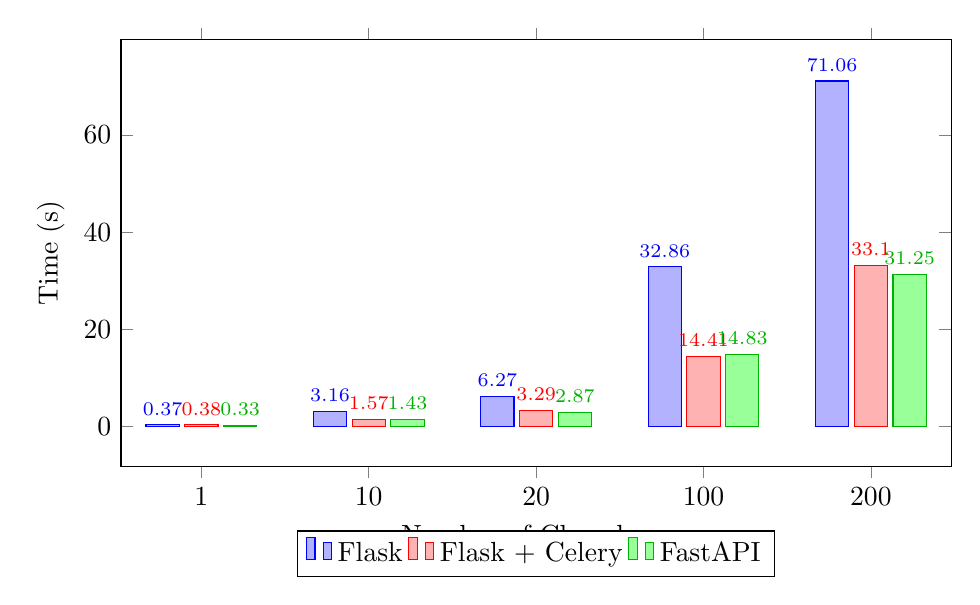
\begin{tikzpicture}
                    \begin{axis}[
                        ybar,
                        bar width=12pt,
                        enlargelimits=0.12,
                        ylabel={Time (s)},
                        xlabel={Number of Cloned \acp{vm}},
                        symbolic x coords={1, 10, 20, 100, 200},
                        xtick=data,
                        legend style={at={(0.5,-0.15)}, anchor=north, legend columns=-1},
                        ylabel near ticks,
                        xlabel near ticks,
                        nodes near coords,
                        every node near coord/.append style={font=\scriptsize},
                        width=1\textwidth,
                        height=7cm,
                    ]

                    % Example dummy data: replace these values with your actual measurements

                    % Flask
                    \addplot+[style={blue, fill=blue!30}] plot coordinates {
                        (1, 0.368690)
                        (10, 3.163624)
                        (20, 6.265722)
                        (100, 32.864042)
                        (200, 71.062075)
                    };

                    % Flask + Celery
                    \addplot+[style={red, fill=red!30}] plot coordinates {
                        (1, 0.377741)
                        (10, 1.565772)
                        (20, 3.287195)
                        (100, 14.412073)
                        (200, 33.095232)
                    };

                    % FastAPI
                    \addplot+[style={green!70!black, fill=green!40}] plot coordinates {
                        (1, 0.330939)
                        (10, 1.434924)
                        (20, 2.872174)
                        (100, 14.832606)
                        (200, 31.253715)
                    };

                    \legend{Flask, Flask + Celery, FastAPI}
                    \end{axis}
                \end{tikzpicture}
                \caption{Execution time to clone increasing number of \acp{vm} across different implementations.}
                \label{fig:cloning_scalability}
            \end{figure}

        \subsubsection{Task 3: VM Deleting}

        



    \subsection{I/O Problems during Batch VM Operations}

        During stress tests of mass cloning and deletion of\ac{vm}s (200 at a time, dispatched to a single\ac{pve} 
        node), we observed rising task times, specifically for the mass cloning of new\ac{vm}s, as can be seen in 
        the following graph

        \begin{figure}[h]
        \centering
        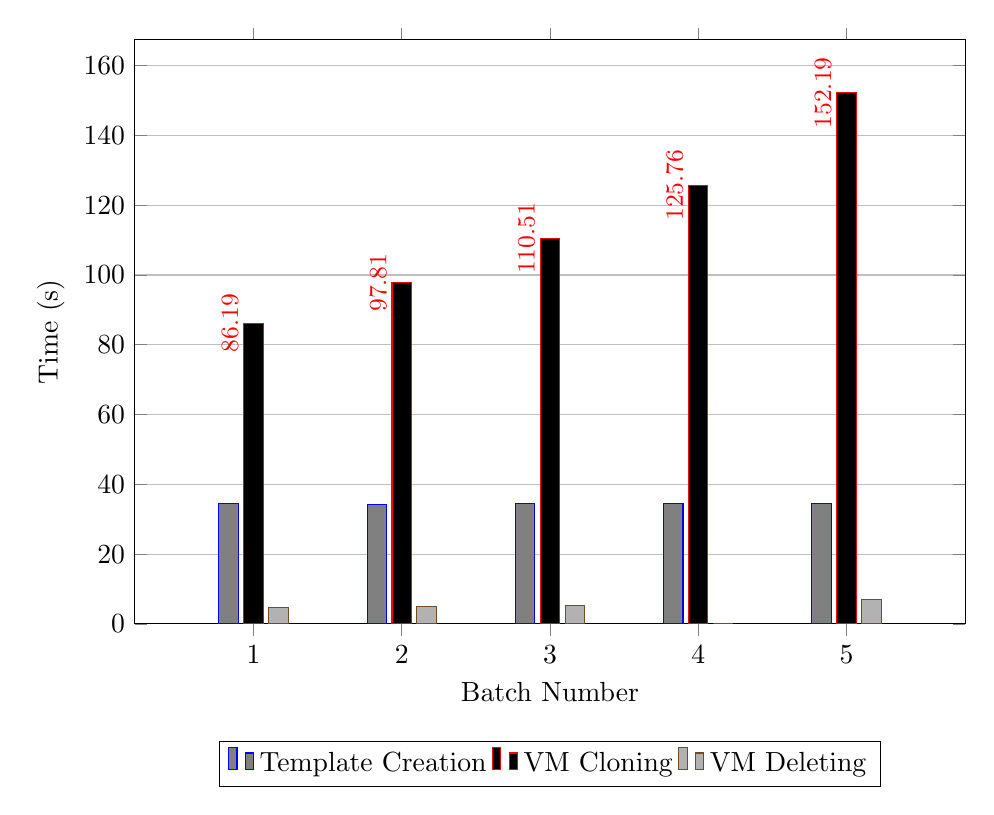
\begin{tikzpicture}
            \begin{axis}[
            ybar,
            bar width=7pt,
            width=\textwidth,
            height=9cm,
            ylabel={Time (s)},
            xlabel={Batch Number},
            symbolic x coords={1,2,3,4,5},
            xtick=data,
            ymin=0,
            enlarge x limits=0.2,
            legend style={at={(0.5,-0.2)}, anchor=north,legend columns=3},
            ymajorgrids=true,
            bar shift auto
            ]

            % Template creation (no labels)
            \addplot+[ybar, fill=gray] coordinates {
            (1,34.379) (2,34.312) (3,34.422) (4,34.609) (5,34.571)
            };
            \addlegendentry{Template Creation}

            % VM cloning (with labels)
            \addplot+[
            ybar,
            fill=black,
            nodes near coords,
            every node near coord/.append style={
                font=\small,
                anchor=south,
                rotate=90,
                yshift=2pt
            }
            ] coordinates {
            (1,86.187) (2,97.805) (3,110.508) (4,125.758) (5,152.186)
            };
            \addlegendentry{VM Cloning}

            % VM deleting (no labels)
            \addplot+[ybar, fill=gray!60] coordinates {
            (1,4.612) (2,4.942) (3,5.377) (4,0.0) (5,7.090)
            };
            \addlegendentry{VM Deleting}

            \end{axis}
        \end{tikzpicture}
        \caption{Grouped bar chart showing VM operation times. Cloning time is labeled to highlight the rising trend. Results
        from Flask running purely sequential code}
        \label{fig:vm_grouped_cloning_focus}
        \end{figure}

        It was also noted that there was an error during the 4th batch of tasks, specifically during the deleting task.

        After some investigation it was found that there were intermittent failures to remove\ac{vm} disks. These failures 
        were \emph{not} detectable via the\ac{pve}\ac{http}\ac{api} responses and only appeared in the\ac{pve} server 
        logs. As orphaned disks accumulated, overall performance degraded significantly.

        \medskip
        \noindent\textbf{Observed Task History Outputs:}
        \begin{verbatim}
--- 1st type of output (VM disks removed successfully) ---
trying to acquire lock...
OK
Logical volume "vm-348786940-disk-0" successfully removed.
TASK OK

--- 2nd type of output (intermittent lock-timeout failures) ---
trying to acquire lock...
Could not remove disk 'local-lvm:vm-120993831-disk-0', check manually:
can't lock file '/var/lock/pve-manager/pve-storage-local-lvm' - got timeout
trying to acquire lock...
OK
Logical volume "vm-120993831-disk-0" successfully removed.
TASK OK

--- 3rd type of output (persistent failures) ---
trying to acquire lock...
Could not remove disk 'local-lvm:vm-363495383-disk-0', check manually:
can't lock file '/var/lock/pve-manager/pve-storage-local-lvm' - got timeout
trying to acquire lock...
can't lock file '/var/lock/pve-manager/pve-storage-local-lvm' - got timeout
TASK OK

--- 4th and final type of output (storage config update errors) ---
trying to acquire lock...
Could not remove disk 'local-lvm:vm-5469324-disk-0', check manually:
can't lock file '/var/lock/pve-manager/pve-storage-local-lvm' - got timeout
trying to acquire lock...
can't lock file '/var/lock/pve-manager/pve-storage-local-lvm' - got timeout
trying to acquire cfs lock 'file-user_cfg' ...
TASK OK
        \end{verbatim}

        This suggests\ac{pve}'s locking mechanism can't keep pace with big amounts of quick sucession delete requests. 
        The lock is used to ensure that two tasks dont modify the\ac{lvm}'s metadata simulatenously. Since there should be 
        some background tasks that are piling up, the system cant keep pace and eventually starts using retries to keep 
        up but even this is insuficient and starts failing more and more towards the end as it becomes fully congested. 
        At the end the system starts becoming overwhelmed and also begins having trouble updating its internal storage 
        config file.  

        This, combined with other factors were the main reason that led us to implement a hard limit on the amount of concurrent 
        requests that can be made from the web application to\ac{pve}\ac{api}. Still, while this significantly reduces the chances 
        of this problem reocurring, it does not fully remedy the problem and additional future work should look into solving this 
        matter completely.

        After performing a cleanup of the orphaned disks we can see that performance was improved from even the 1st baseline test.

        \begin{figure}[h]
        \centering
        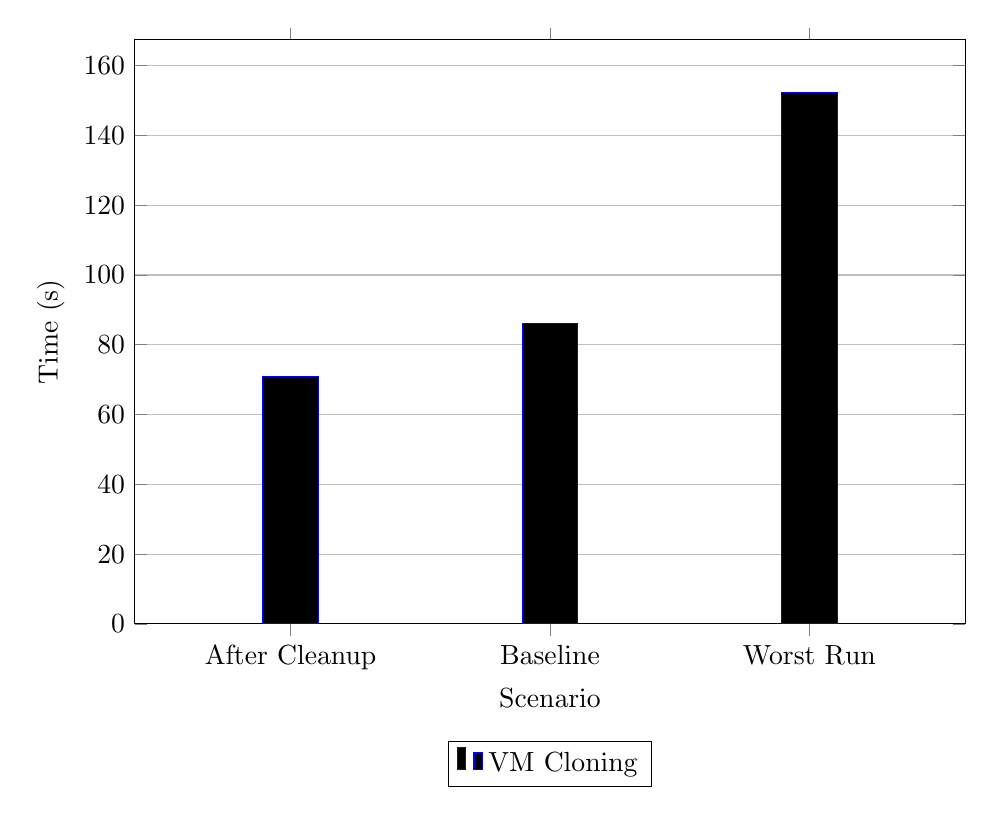
\begin{tikzpicture}
            \begin{axis}[
                ybar,
                bar width=20pt,
                width=\textwidth,
                height=9cm,
                ylabel={Time (s)},
                xlabel={Scenario},
                symbolic x coords={After Cleanup, Baseline, Worst Run},
                xtick=data,
                ymin=0,
                enlarge x limits=0.3,
                legend style={at={(0.5,-0.2)}, anchor=north, legend columns=1},
                ymajorgrids=true
            ]

            % VM cloning bars without labels
            \addplot+[
                ybar,
                fill=black
            ] coordinates {
                (After Cleanup,70.954)
                (Baseline,86.187)
                (Worst Run,152.186)
            };
              
            \addlegendentry{VM Cloning}

            \end{axis}
        \end{tikzpicture}
        \caption{Bar chart showing VM cloning times after cleanup, at baseline, and in the worst case scenario.}
        \label{fig:vm_grouped_cloning_focus}
        \end{figure}




% Write text in here
% Use \subsection and \subsubsection to organize text

